% RQ3
\section{Ranking}
\label{sec:toolranking}
% Most important:
% Finding the top performing tool is most important, then low MSE for that top performing
% Confidence in automation
% 

Now that a predictor for future error detection tool performance is introduced, the goal of an estimated ranking of tools with respect to their performance will be discussed.
~\\As an absolute score is helpful to know with a single tool at your disposal, a ranking or recommendation of tools and their strategies would be of greater use for the end-user. The question proposed here is to see if such a ranking could be made, ranking the better performing tools higher in the ranking. This also allows for other metrics to experiment with. The regressors (estimators) used in section \ref{sec:performanceprediction} could now also be optimized using information retrieval ranking scores. This might result in different distinguishing features found by the regression models and shows the possible flexibility of these models (if it is possible to get good rankings).
The flow of the ranking is shown in figure \ref{fig:method_ranking}.

\begin{figure}
    \centering
    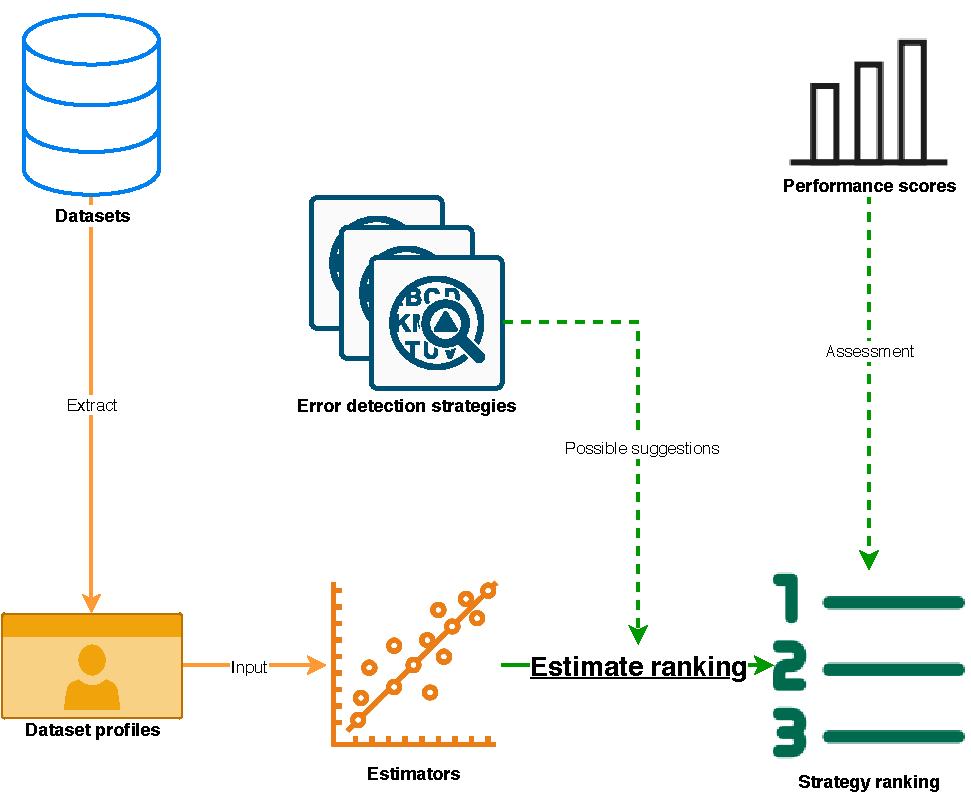
\includegraphics[width=0.9\textwidth]{thesis/Figures/Method/PerformanceEstimation-Ranking.pdf}
    \caption{Flow of the estimation of strategy ranking}
    \label{fig:method_ranking}
\end{figure}

\subsection{Method of ranking}
A user should be able to retrieve an estimated ranking of high performing strategies without running these tool on an unseen dataset. A ranking should be $K$ strategies long, with a predefined $K$. It should be so that a user can a variety of tools and configurations to pick from. For this research, a $K$ of 10 will be used. 10 is the number of search suggestion in the basic Google search bar\footnote{\url{https://www.google.com/}}. However, this value can be altered to the users preference.
\\Besides the number of strategies that should be returned, it is also worth considering that there should be a limit on the total number of strategies per tool should be returned. As there are many configurations for each tool, certain configurations might not differ too much in the inner workings and end results. So, a limit $L$ is used to limit the number of configurations per tool. This makes the minimum of different tools, suggested in a ranking of size $K$, the ceiling function of $K$ divided by $L$: $\ceil{\frac{K}{L}}$. 
\\It should be possible to generate ranking according to each of the scores that the estimators are capable of predicting. So not only an F1-score based ranking, but also precision and recall. Users then will be able to decide which strategy should be picked for which job.
\\To generate an estimated ranking for a new unseen dataset, the data profile as described in section \ref{subsec:dataprofiles} is created. Then all estimators configured with the best configuration as found by section \ref{subsec:estimatorselection} are given this data profile as input, generating estimated scores for all strategies $s \in S$. These estimated scores (like a single column in table \ref{tab:estimatedscores}) are then sorted, and for each tool, only $L$ rows are kept. Then the top $K$ rows will be returned. An example of this can be shown in tables \todo{Tabels}


\begin{table}[]
\centering
\begin{tabular}{|l|l|l|l|}
\hline
\textbf{Rank} & \textbf{Tool} & \textbf{Configuration} & \textbf{Estimated F1} \\ \hline
1             & Tool 1        & Config 1-a             & $\hat{y}(s_{1-a}, d)$ \\ \hline
2             & Tool 2        & Config 2-a             & $\hat{y}(s_{2-a}, d)$ \\ \hline
3             & Tool 3        & Config 3-a             & $\hat{y}(s_{3-a}, d)$ \\ \hline
4             & Tool 4        & Config 4-a             & $\hat{y}(s_{4-a}, d)$ \\ \hline
5             & Tool 5        & Config 5-a             & $\hat{y}(s_{5-a}, d)$ \\ \hline
6             & Tool 6        & Config 6-a             & $\hat{y}(s_{6-a}, d)$ \\ \hline
\end{tabular}
\caption{Strategy ranking for best tool}
\label{tab:ranking_best_tool}
\end{table}


\begin{table}[]
\centering
\begin{tabular}{|l|l|l|l|}
\hline
\textbf{Rank} & \textbf{Tool} & \textbf{Configuration} & \textbf{Estimated F1} \\ \hline
1             & Tool 1        & Config 1-a             & $\hat{y}(s_{1-a}, d)$ \\ \hline
2             & Tool 1        & Config 1-b             & $\hat{y}(s_{1-b}, d)$ \\ \hline
3             & Tool 1        & Config 1-c             & $\hat{y}(s_{1-c}, d)$ \\ \hline
4             & Tool 1        & Config 1-d             & $\hat{y}(s_{1-d}, d)$ \\ \hline
5             & Tool 1        & Config 1-e             & $\hat{y}(s_{1-e}, d)$ \\ \hline
6             & Tool 1        & Config 1-f             & $\hat{y}(s_{1-f}, d)$ \\ \hline
7             & Tool 1        & Config 1-g             & $\hat{y}(s_{1-g}, d)$ \\ \hline
8             & Tool 1        & Config 1-h             & $\hat{y}(s_{1-h}, d)$ \\ \hline
9             & Tool 1        & Config 1-i             & $\hat{y}(s_{1-i}, d)$ \\ \hline
10            & Tool 1        & Config 1-j             & $\hat{y}(s_{1-j}, d)$ \\ \hline
\end{tabular}
\caption{Strategy ranking for best configuration per tool}
\label{tab:ranking_best_configuration}
\end{table}

\subsection{Performance measure of ranking}
To analyze the results of the produced rankings, the ranked strategies of first will be qualitatively be addressed. Generating actual lists of suggested error detection strategies to use and glancing over them will give a first indicates on whether the results will be promising.
\\Then of course, more quantitative metrics will be calculated to compare and analyze the results of these rankings. Precision, recall and f-score are possible to be calculated, but the assumption with those metrics in ranking results, is that the return list is an unordered set of documents (suggestions).
Average Precision is a metric that takes into account the ranking of the returned documents as well. Unfortunately, this metric uses a binary relevance scoring, where the last relevant document is equally important to rank high as the first relevant document. In this research, a cutoff point for a score should then be chosen to evaluate, for example, any strategy with a score > 0.5 would be considered relevant. Taking the mean average precision for all different unseen datasets and the produced rankings would then have some meaning, but does not fit this purpose best.

~\\A metric that does take the relative importance into account, is the discounted cumulative gain (DCG). It allows degrees of relevance, which is suited for our purpose. The top ranks count the most, meaning whenever a highly relevant (high scoring strategy) is actually listed at the top, the DCG reflects that in a positive way. The utility also decreases with the rank, meaning that lower ranks count less towards the DCG. The DCG is a summation of the relevance score discounted by a log value relative to the given place in the ranking (shown in equation \ref{eq:DCG}).
~\\Also, a normalized version of the discounted cumulative gain exists. It takes the ideal ranking and calculates the DCG ($IDCG_k$). The output metric will be the $DCG_k$ for the produced ranking, divided by the DCG for the best ranking (see equation \ref{eq:NDCG}). 

\begin{equation}
\label{eq:DCG}
    DCG_k = \sum^k_{r=1} \frac{rel_r}{\log(r+1)}
\end{equation}

\begin{equation}
\label{eq:NDCG}
    NDCG_k = \frac{DCG_k}{IDCG_k}
\end{equation}

The relevance of a return item in a ranking must be determined beforehand. It should have a relation to how good a strategy performs. 
That is why for this research, the actual real score of a strategy run on a specific dataset will be the relevance. Not only allows this for automatic relevance estimation, but also it gets rid of the problem of distinguishing between two or more very similar strategies, that would maybe not make the list due to the limits set on strategies per tool $L$ and the size of the ranking $K$.

